代码见附件中的simplex文件夹, 或GitHub的备份\footnote{
    \href{https://github.com/ikaroinory/convex-opt/tree/main/homework/homework1/simplex}{https://github.com/ikaroinory/convex-opt/tree/main/homework/homework1/simplex}
}.
运行结果如\cref{figure:14-1}所示.

\begin{figure}
    \centering
    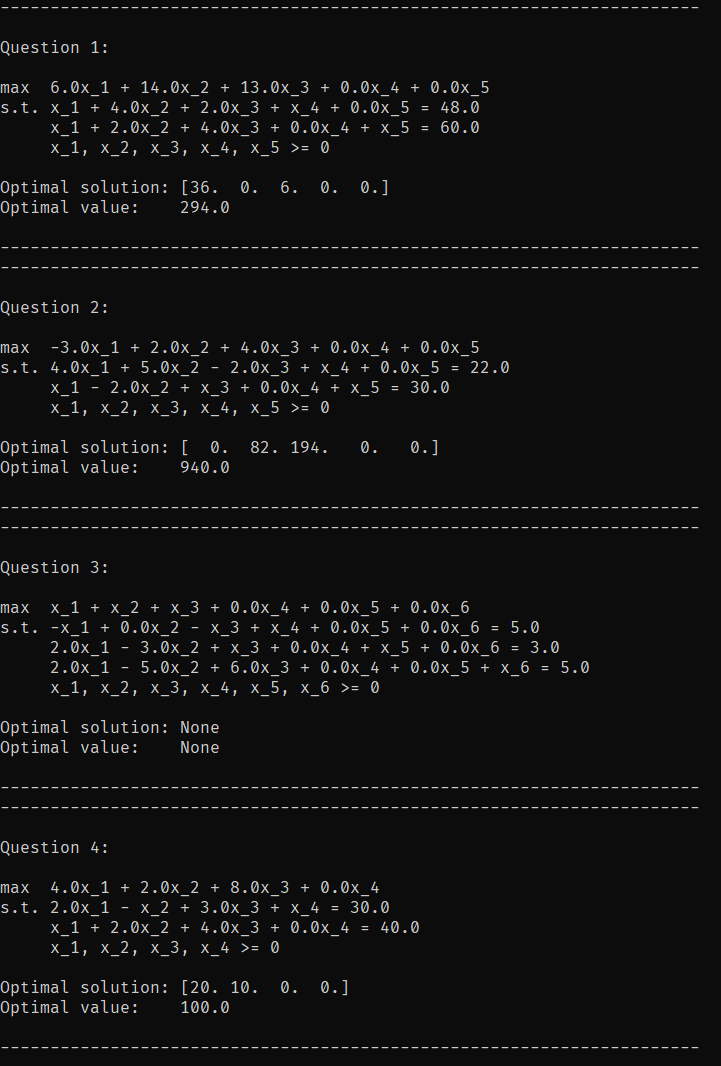
\includegraphics[width=\textwidth]{figures/14-1.png}
    \caption{程序simplex/main.py的输出}
    \label{figure:14-1}
\end{figure}
